\documentclass[fleqn]{beamer}
\title{Contextualism in Relativity and Quantum~Theories}
\author{Hans Halvorson}
\date{October 19, 2023}
\providecommand{\tightlist}{%
  \setlength{\itemsep}{0pt}\setlength{\parskip}{0pt}}
\usepackage{tikz}
\usepackage{tikz-cd}
\tikzcdset{scale cd/.style={every label/.append style={scale=#1},
    cells={nodes={scale=#1}}}}

\usetikzlibrary{calc}
\usepackage{pgfplots}
\usetheme{Copenhagen}
\useoutertheme{infolines}
\setbeamertemplate{navigation symbols}{}
% \usepackage{quiver}
\begin{document}

\begin{frame}[plain]

  \titlepage

\end{frame}


\begin{frame}[plain]{Abstract}

  I review two accounts of global reference frames in spacetime
  theories (and Einstein's special theory of relativity in
  particular):

  \begin{enumerate}
  \item Absolutism: All fundamental facts are frame-independent, and
    the frame-relative facts are derivable from them.
  \item Fragmentalism: All fundamental facts are frame-relative, and
    there are no non-trivial logical relations between the facts in
    one reference frame and the facts in another reference frame.
  \end{enumerate}

  I argue that both of these accounts are fatally flawed, and I
  develop an alternative account that builds on the intuitions behind
  these other accounts. (I also consider the relation between these
  accounts and methodological imperatives regarding ``good physics''.)
  Finally I consider whether this sharpened account of contextualism
  in relativity theory can shed light on the sort of contextualism
  that we encounter in quantum theories.

\end{frame}

\begin{frame}[plain]{Overview}

  \tableofcontents

\end{frame}


\section{Contextual realism?}

\begin{frame}

  \begin{itemize}
  \item Scientific realism is typically factored into two components:
  \begin{enumerate}
  \item Semantic: Interpret the statements of the theory literally
  \item Epistemic: Believe \textit{all} of the statements of the
    theory
  \end{enumerate}
  
\item Hidden third component: How is a theory supposed to be related
  to its user?

  \begin{enumerate}
  \item Context insensitivity: The theory consists of representational
    items (e.g.\ sentences, propositions, models) that are intended to
    represent universal truths.
  \item Context sensitivity: A theory is a function from contexts to
    descriptions, where the context is supplied by the user.
  \end{enumerate}
  
\end{itemize}

\end{frame}



\begin{frame}{ }

  \begin{itemize}

  \item Contemporary physical theories display contextualism of model
    choice.
    \begin{itemize}
    \item There is no single model of GTR that is most adequate to
      reality.
    \item There is no single model of QM that is most adequate to
      reality.
   \end{itemize}
 \item However, this contextualism of model choice is, in principle,
   eliminable.
 \item Today's question: Are our best theories \textbf{intrinsically
     contextual} --- i.e.\ the truth is not contained in the theory
   per se, but in the beliefs formulated by contextually bound users.
   \begin{itemize}
   \item STR: The truth is not in the frame-independent, 4d model, but
     in the frame-relative 3+1 descriptions.
   \end{itemize}
  \end{itemize}
\end{frame}




\section{Theory of Relativity or Theory of Invariants?}

%% tikz dialectical spiral

\begin{frame}

\begin{tabular}{l c c c}
  & relativism & & absolutism \\ \hline
  & Berkeley & & \\
  & Mach & & \\
  & Avenarius & & \\
  1905 & & \textbf{STR}  \\
  1908 & Petzoldt & & Minkowski \\
  1915 &          & \textbf{GTR} & \\
  1917 & Schlick  & & \\
  1920 &          & & Einstein \\
       &          & & Eddington \\
  1960 &          & & Putnam \\
  2005 & K.\ Fine & &   \\
       & H. Brown & & Balashov      \\
       & Rovelli  & & Hofweber \& Lange \end{tabular}


\end{frame}





\section{Review: Special Theory of Relativity}

  
\begin{frame}{Review of STR}

 \begin{center}
 \begin{tikzpicture}[scale=1]
   \draw[->,red] (0,-3)--(0,3) node[left]{Alice};
   \draw[-,red] (-3,0)--(3,0);
   \draw[->,blue] (-1,{-sqrt(10)})--(1,{sqrt(10)}) node[right]{Bob}; % 1,sqrt(10)
   \draw[blue] ({-sqrt(10)},-1)--({sqrt(10)},1);
   \draw[domain=-1:1,dashed,smooth,variable=\t] plot ({cosh(\t)},{sinh(\t)});
 \end{tikzpicture}   
\end{center}


 
\end{frame}

\begin{frame}

 \begin{center}
 \begin{tikzpicture}[scale=5]
   \draw[->,green] (0,-0.5)--(0,0.5);
   \draw[->,green] (1,-0.5)--(1,0.5);
   \draw[-,red] (0,0)--(1,0);
   \draw[blue] (0,0)--({sqrt(10)*2/6},2/6);
   \draw[domain=0:0.35,dashed,smooth,variable=\t] plot ({cosh(\t)},{sinh(\t)});
 \end{tikzpicture}   
\end{center}  


\end{frame}

\begin{frame}{Frame-dependent and frame-independent facts}

  \begin{itemize}
  \item Proper length: The extension of a family $\Gamma$ co-moving
    particles in their own frame of reference
  \item Length contraction: The length of the intersection of $\Gamma$
    with an arbitrary spacelike hypersurface (never longer than proper
    length)
  \item Shape relativity: the intersection of $\Gamma$ with
    $\Sigma _1$ might have different geometric properties than the
    intersection of $\Gamma$ with $\Sigma _2$.
    \begin{itemize}
    \item E.g.\ an isosceles triangle in one frame but not in another
    \end{itemize}
  \item Spacetime distance
    \begin{itemize}
    \item Non-unique decomposability
    \end{itemize}
  \end{itemize}
  
\end{frame}

\begin{frame}{Eddington's IBE}

    \begin{tabular}{cl}
         \begin{tabular}{c}
           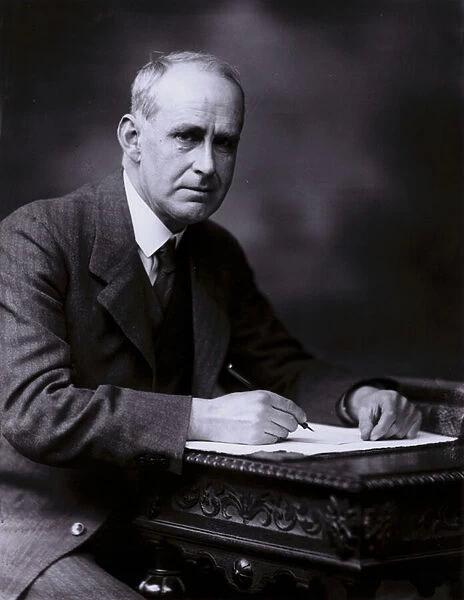
\includegraphics[height=3.75cm, width=2.75cm]{eddington} \\
           Arthur Eddington \\
           (1882--1944)
           \end{tabular}
      & \begin{tabular}{l}
          \parbox{0.6\linewidth}{\small %  change the parbox width as
            % appropiate
          ``[A]n observer on the earth sees and measures an oblong block; an
          observer on another star contemplating the same block finds it to be
          a cube. Shall we say that the oblong block is the real thing, and
          that the other observer must correct his measures to make allowance
          for his motion? All the appearances are accounted for if the real
          object is the four-dimensional, and the observers are merely
          measuring different three-dimensional appearances or sections; and
          it seems impossible to doubt that this is the true explanation.''
          }
         \end{tabular}  \\
  \end{tabular}

\end{frame}


\begin{frame}{ }

  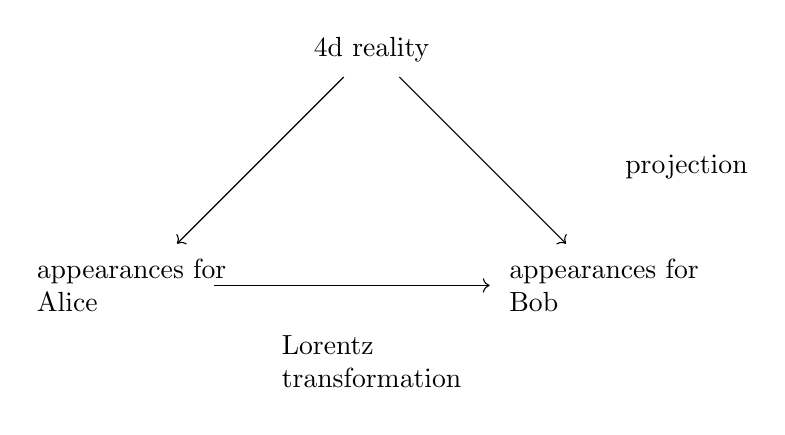
\begin{tikzpicture}
    \node[] at (0,3) {4d reality};
    \node[] at (-3,0) [text width=2.5cm]{appearances for Alice};
    \node[] at (3,0) [text width=2.5cm]{appearances for Bob};
    \node[] at (4,1.5) {projection};
    \node[] at (0,-1) {\begin{tabular}{l} Lorentz \\ transformation \end{tabular}};
    \draw[->,shorten >=0.75cm,shorten <=0.5cm] (0,3)--(-3,0);
    \draw[->,shorten >=0.75cm,shorten <=0.5cm] (0,3)--(3,0);
    \draw[->,shorten >=1.5cm,shorten <=1cm] (-3,0)--(3,0);
  \end{tikzpicture}

\end{frame}  


\section{Fragmentalism}

\begin{frame}{Early reception of STR}

  \begin{tabular}{cl}
         \begin{tabular}{c}
           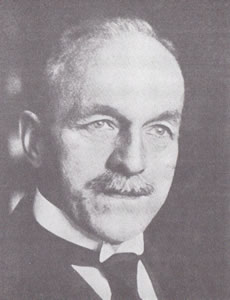
\includegraphics[height=4cm, width=2.75cm]{petzoldt} \\
           Joseph Petzoldt \\
           (1862--1929)
           \end{tabular}
    & \begin{tabular}{l}
        \parbox{0.6\linewidth}{%  change the parbox width as
                               %  appropiate
        ``We can only think of things just as we find them and not as no-one
        finds them. We can only ever think of them from the perspective in
        which we find them, and not from a perspective from which we cannot
        think of them, or in general from no perspective at all. There is no
        absolute perspective and there is no absence of perspectives, there
        are only relative perspectives.'' (1906, p 142-43)
        }
         \end{tabular}  \\
  \end{tabular}

  

\end{frame}


\begin{frame}{Fragmentalism}

  \begin{itemize}
  \item Kit Fine (2005) wants to be a \textbf{realist about tense}:
    tensed statements are simply true or false --- not true or false
    relative to some point of time.

    \smallskip ``Albert Einstein is alive.''

  \item Fine's solution is that reality consists of temporal fragments
    which are internally coherent, but incoherent with each other.

  \item Fine then applies this idea to STR: reality consists of
    frame-time fragments, i.e. one for each spatial hyperplane in
    Minkowski spacetime

  \end{itemize}

\end{frame}

\begin{frame}{Fragmentalism}


[TO DO: insert picture illustrating fragmentalism]

\end{frame}



\section{The revenge of absolutism}


% \begin{tikzcd}[ampersand replacement=\&]
% 	\&\&\& {\text{4d reality}} \\
% 	\\
% 	\\
% 	{\text{appearances} \\ \text{for Alice}} \&\&\&\&\&\& {\text{appearances} \\ \text{for Bob}}
% 	\arrow[squiggly, from=1-4, to=4-1]
% 	\arrow["{\text{projection}}", squiggly, from=1-4, to=4-7]
% \end{tikzcd}

\begin{frame}{Hofweber and Lange}

  ``\dots what is radical about fragmentalism is that it regards both
  of them as \textit{fundamental} rather than as derivative from a
  more fundamental reality consisting of facts that are invariant
  across different (frame-)times.'' (p 874)

\end{frame}

\begin{frame}{Hofweber and Lange}

  ``The standard interpretation of STR is not merely that the facts
  associated with different inertial frames are on a par, but also
  that they are not fundamental. Instead, `tenseless' facts about
  four-dimensional Minkowski spacetime are fundamental, and their
  `tensed' projections onto various reference frames are derivative
  from them.'' (p 874)

\end{frame}

\begin{frame}{Hofweber and Lange}

  ``If reality consists fundamentally of `fragments' corresponding to
  the facts that hold relative to frame-times, then there is no reason
  for there to be laws relating the facts that these different
  fragments contain. On the other hand, if the tensed facts in these
  fragments are instead projections onto various reference frames of
  tenseless facts about four-dimensional Minkowski spacetime, then
  there is every reason to expect there to be laws relating facts in
  different frames, since those laws govern the way in which the
  four-dimensional reality is projected onto different spacetime
  coordinate systems.'' (p 874)

\end{frame}



\begin{frame}{Hofweber and Lange}

  ``What explains this systematic connection between length and
  relative movement? The standard explanation is that a single
  4-dimensional reality with an invariant spacetime interval presents
  itself in different frames as separating differently into space and
  time.'' (p 879)
  

\end{frame}


\begin{frame}{Central doctrines of absolutism}

  \begin{itemize}
  \item Only \textbf{invariant quantities} are physically significant

    \medskip ``The spacetime interval is frame-invariant and is more
    fundamental than any frame-dependent fact.'' (p 875)
    
    \smallskip ``Invariants -- quantities that everybody agrees on
    regardless of their frame of reference -- play a more important
    role in our understanding of the world than quantities that vary
    from one frame of reference to another.'' (Mermin 2009: 79)
    
  \item A fundamental theory would be formulated in terms of
    \textbf{frame-independent} quantities. The notion of a
    \textbf{frame of reference} would first come up in applying the
    theory.

  \end{itemize}
\end{frame}

\begin{frame}{Central doctrines of absolutism}

  \begin{itemize}
    
  \item To justify belief that (or explain why) two descriptions $D_1$
    and $D_2$ are equivalent, one must produce a third, and more
    fundamental, description $D$

    \medskip ``To support a claim of equivalence between a pair of
    theories, stated in a pair of languages in which mass is described
    using different units, we brought in a third language, a language
    in which mass is described in a unit-free way, using the concepts
    $\succeq$ and $C$. This third, more fundamental, language gave us
    a perspective on the fundamental facts, a perspective from which
    the first two theories could be seen as getting at the very same
    facts.'' (Sider 2020, p 187)
  \end{itemize}


\end{frame}



\section{Objectivity without absolutism}





\begin{frame}{Agreement with Hofweber and Lange}

  \begin{itemize}
  \item Fragmentalism fails to recognize --- not to speak of explain
    --- the fact that there are non-trivial relations between the true
    descriptions in different frames of reference.
  \item $[A=a_1]_{F_1}$ is \textbf{compatible} with $[A=a_2]_{F_2}$
    \begin{itemize}
    \item \item Fine thinks that indexing attributions to frames is
      not realist enough. So he claims that they are inconsistent
      facts. \end{itemize}
    \begin{itemize}
    \item Hofweber and Lange claim that these two ``appearances'' are
      not inconsistent \textit{because} they are caused (?) by the
      same frame-independent object.
    \end{itemize}
  \item $[A=a_1]_{F_1}$ is \textbf{p-equivalent} to $[A=a_2]_{F_2}$.
  \item According to a standard account of facts, $[A=a_1]_{F_1}$ is
    \textbf{the same fact} as $[A=a_2]_{F_2}$.
  \end{itemize}


\end{frame}


  %   \begin{itemize}
  %   \item How are we to understand these relations?
  % \item A simple proposal: the two observers are talking about the
  %   same facts. But there is no ``third person'' to state these facts
  %   in a frame-independent fashion
  % \end{itemize}



\begin{frame}{Covariance}

\begin{center}
\begin{tikzcd}[ampersand replacement=\&]
  A  \arrow[dd] \arrow[rr] \& \& B  \arrow[dd] \& \& \text{change of context} \\ \\
  D_A \arrow{rr}[swap]{\begin{array}{c} \text{Lorentz} \\
      \text{transformation}\end{array}} \& \& D_B \& \& \text{change
    of description}
\end{tikzcd}
\end{center}

\end{frame}


\begin{frame}{Critique of absolutism}

  \begin{itemize}
  \item Hofweber and Lange: the relation between frame-relative
    statements is mediated by their both being ``projections'' of some
    four-dimensional statement.
  \item What is this relation of ``projection'' supposed to be?
    \begin{itemize}
    \item The absolutists are borrowing causal terminology from
      everyday life and dynamical theories. E.g.\ a shadow is caused
      by the rabbit.
    \item But we lack a theory of how 4d timeless entities can cause
      3d objects to exist.
    \item In fact, the timeless nature of 4d objects seems to
      disqualify them from playing a causal role in the normal sense
      of the word (where \textit{changes} in one object lead to
      changes in another).
    \item In what sense are 3d objects ``appearances''?  What is the
      mechanism by which these appearances are generated?
    \end{itemize}
  \end{itemize}


\end{frame}

\begin{frame}{Critique of absolutism}

  \begin{itemize}
  \item Each frame-relative description (if we inclue both position
    and momentum) is logically complete.
    \begin{itemize}
    \item Unlike the relation between 2d projections and 3d objects,
      the frame-relative descriptions are not logically weaker than
      the 4d description.
    \end{itemize}
  \item The desire to explain relations in terms of something
    intrinsic is characteristic of various absolutisms.
    \item The demand for an ontological explanation of transformation
    rules would show that Galilean relativity is intrinsically
    four-dimensional.
    \begin{itemize}
    \item But the standard explanation of Galilean relativity is the
      \textit{absence} of a preferred reference frame. \end{itemize}
  
  \end{itemize}

\end{frame}

\begin{frame}{A merely verbal dispute?}

  \begin{itemize}

  \item Lange: The four-dimensional affine space $M$ is a first-order
    representation of reality (as it is in itself)

  \item Halvorson: The four-dimensional affine space $M$ is a
    ``symbolic form'' that permits the creation and coordination of
    first-order representations of reality

  \item If there are rules for transforming between true descriptions,
    then what difference does it make whether we have a ``picture'' of
    a more fundamental reality?

    \begin{itemize}
    \item Does believing that $M$ itself represents have any more
      content then believing that the Lorentz transformations are
      correct? \end{itemize}

  \end{itemize}

  

\end{frame}

\section{Quantum contextualism}


\begin{frame}{Problem of the preferred basis}

  \begin{itemize}

  \item A quantum state $\psi$ is a function $A\mapsto \psi |_A$ from
    maximal quantities to probability distributions over outcomes:
    \[ \langle \psi ,A\psi \rangle \: =\: \sum _{i=1}^n a_i\langle
      \psi ,E_i\psi \rangle .\]

  \item Quantum contextualism (inspired by Niels Bohr and Grete
    Hermann): The describer is free to choose his context, represented
    by a preferred observable $A$.

    \begin{itemize}
    \item Bohr: The notion of a measurement context generalizes the
      notion of a frame of reference.
    \end{itemize}

  \end{itemize}

\end{frame}


\begin{frame}{Is QM radically contextual?}
  
\begin{itemize}  

\item The distribution $\psi |_A$ is compatible with the distribution
  $\psi |_B$ in the sense that they arise from the common state
  $\psi$.

\item Failure of covariance: the distribution $\psi |_B$ cannot be
  derived from the distribution $\psi |_A$.
  \begin{itemize}
  \item Perhaps we need to include information about derivatives of
    the distribution?
  \end{itemize}

\item Subjectivity of outcomes: an ignorance interpretetation of
  $\psi |_A$ is incompatible with an ignorance interpretation of
  $\psi |_B$.

  \begin{itemize}
  \item The no hidden variables theorems (e.g.~Kochen-Specker) show
    that there is no consistent, non-contextual assignment of
    properties that reproduces the quantum statistics.
  \end{itemize}
  
\end{itemize}

\end{frame}


\begin{frame}{The ambiguous role of context}

  Does context describe the physical state of the subject
  (mechanical), or the mental frame of the subject (semantic)?

  \begin{itemize}
  \item Semantic: The agent's choice of context for description
    changes nothing in the object being described.
    \begin{itemize}
    \item Example: Changing the language used to describe an object.
    \item Example: Changing from one inertial frame of reference to
      another.
    \end{itemize}
  \item Mechanical: An agent's ``context'' is just another word for
    her physical state.
    \begin{itemize}
    \item A change of the agent's state can alter the object's
      state. (Bohm, Rindler)
    \item An agent's state, and its relation to the object's state,
      are subject to the laws of the theory.
   \end{itemize}
  \end{itemize}

\end{frame}


\begin{frame}{Problem of the preferred basis}

  \begin{itemize}
  \item Two ways to explain away the freedom of the experimenter:

    \begin{enumerate}
    \item Position fundamentalism (GRW, Bohm)
    \item Dynamical basis selection, e.g.\ via decoherence
    \end{enumerate}
     
  \item Fact: Bohmian mechanics reproduces Bohr's contextualism via
    the free choice of a Hamiltonian that correlates a preferred
    observable $R$ with position $Q$.
    \begin{itemize}
    \item Bohmian mechanics has no explanation for why one Hamiltonian
      applies rather than another.
    \end{itemize}

  \item Claim: The selection of preferred basis via decoherence is a
    pretense of an explanation (for determinacy), when there actually
    is a free variable that we set by hand. (See A. Fine, ``With
    complacency or concern: solving the quantum measurement
    problem''.)
  \end{itemize}

\end{frame}

\begin{frame}{Conclusion}

  \begin{itemize}
  \item The idea that absolutism is epistemically unwarranted and even
    politically bad drove the thinking of Berkeley, Mach, and
    Petzoldt, among others.
  \item The idea that relativism is cowardly and even politically bad
    drives the thinking of modern scientific realists.
    \begin{itemize}
    \item R1: An objective description is a description of things as
      they are in themselves.
    \item R2: The mathematical theory of invariants gives us a grip on
      things as they are in themselves.
    \end{itemize}
  \end{itemize}

\end{frame}

\begin{frame}{Conclusion}

  \begin{itemize}
  \item The attempt to synthesize conflicting intuitions about reality
    and human representation drove Kant to the idea that:
    \begin{itemize}
    \item There is mind-independent reality.
    \item No human description is mind-independent.
    \end{itemize}
  \item Kant's successors couldn't maintain the tension.
    \begin{itemize}
    \item Skepticism
    \item Dogmatism: Hegel contra Kant: I can transcend
      context-dependence. Thought has become one with Reality.
    \end{itemize}
  \end{itemize}  

  \end{frame}

  \begin{frame}{Conclusion}
  \begin{itemize}
  \item The requirement of \textbf{covariance of descriptions} is
    tantamount to the belief that there is an objective reality to
    which our mind-dependent representations must answer.
  \item The frame-dependent descriptions in STR are complete physical
    descriptions, and completely equivalent to each other.
  \item QM appears to be more radically contextual than STR.
  \item QM forces us to reconsider the idea that context is purely
    semantic.
  \end{itemize}

\end{frame}

\end{document}


 \begin{frame}{Questions}

\begin{itemize}
\item Given a contextual theory \(T\), shouldn't there be a
  non-contextual theory \(T'\) from which \(T\) can be derived?
\end{itemize}
\end{frame}


\begin{frame}{The Big Question}
\begin{itemize}
\item Many traditional realists would assume that \textbf{ineliminable
    perspectivalism} is inconsistent with scientific realism

  \begin{itemize}
  \tightlist
\item Ineliminable perspectivalism: the perspective-bound facts cannot
  be derived from absolute facts
  \end{itemize}
\item Question: Can a scientific theory be ``good enough'' if it is
  ineliminably perspectival, i.e.~if it fails to provide a core of
  absolute truths?
\end{itemize}

picture

\begin{itemize}
\item Is ``find a coordinate free formulation'' an epistemic
  imperative?
\item Is ``find a gauge free formulation'' an epistemic imperative?
\end{itemize}
\end{frame}

\begin{frame}{Coordinates and reference frames}
\begin{itemize}
  \tightlist
\item
  How should we think of computing \emph{invariants}?
\end{itemize}
\end{frame}


\begin{frame}{Contextualism versus Perspectivalism}
\begin{itemize}
\item Example(s): perspective in everyday life

  \begin{itemize}
  \item shapes appear differently to people standing in different
    places
  \item colors appear differently to people to people relative to
    different background lighting conditions
  \end{itemize}
\item Example: three-dimensional shape projected onto two-dimensional
  surfaces
\item Example: centering features


  \begin{itemize}
  \item Should STR serve as a template for future physical theories?
  \end{itemize}
\item Sider's criterion for equivalence of descriptions
\end{itemize}
\end{frame}

\begin{frame}{Unremarkable contextualism}
  \begin{itemize}
  \item Compare with Gil Harman
  \end{itemize}
\end{frame}




%%% Local Variables:
%%% mode: latex
%%% TeX-master: t
%%% End:
